Simply because a synchronization protocol is ideal at the start of the simulation, does not mean that it will still be ideal during the simulation.
It is well known, and repeated in the previous section, that model behaviour significantly influences the ideal synchronization protocol.
Contrary to many modelling formalisms, the \textsf{DEVS} formalisms makes it possible to model basically any kind of discrete event model.
As such, it is possible for the model to significantly change its behaviour throughout the simulation.

Defining the ideal synchronization protocol at the start of the simulation, when information about future model behaviour is scarce, might therefore not offer the best possible performance.
In \textit{dxex}, we not only make it possible to define the synchronization protocol to use, but also to change this decision throughout simulation.
To do this, all kernels are notified of the switch and they are forced to stop simulation.
When stopped, each kernel instantiates a new core, with the new synchronization protocol, that is provided with the simulation state of the previous core.
Simulation is then resumed with the new cores after the previous ones are destroyed.

As usual, switching imposes an overhead and should thus only be done if the benefits outweigh the induced overhead.
This overhead depends on the size of the model and the number of simulation cores.
For a simple model and a few cores, the overhead is less than a second.

Although we currently only support manual switches between different synchronization protocols, this is not necessarily the case.
Ideally, a new component is added to the simulation kernel, which monitors model behaviour and simulation performance, and toggles between them automatically.
Our interface is augmented with the necessary bindings for such a decision component.
Also, our interface is augmented with an interface for statistics gathering and model behaviour analysis.
The implementation of such a component is currently left open, but we envision algorithms heavily based on machine learning.

\subsection{Statistics Gathering}
Traditionally, models are not exposed to simulation kernel details due to the wrong level of abstraction.
Simulation models only care about being simulated, and not about how this is being done.
This is different for a new simulation kernel component that has to monitor the behaviour of not only the model, but the simulator as well.

We add performance metrics in the simulation kernel, which logs relevant performance metrics and processes them for use in other components.
These metrics include the number of events created and destroyed, the number of inter- and intra-kernel events, the number of rollbacks, the measured lookahead, details of the Global Virtual Time (GVT) and Earliest Output Time (EOT) calculations, and information on the fairness between simulation kernels.
With all these metrics, a component can get a fair view on both model and simulation kernel behaviour.

For example, if the actually seen lookahead is significantly higher than the defined lookahead, it might be interesting to switch to optimistic synchronization.
When the number of rollbacks is excessively high, switching to conservative synchronization might be considered.
%And when neither of these two is an option, the simulation might just (temporarily) have to fall back to sequential simulation. % Falling back to sequential is not supported atm.

\subsubsection{Visualization of Communication}
To provide more insight in our benchmark models, we created a simple visualization of their simulation trace.
This trace visualizes the allocation of the model and all defined connections.
For each connection, the number of events transferred is annotated.
Examples are shown for the three benchmark models used before: Figure~\ref{fig:Queue_allocation}, Figure~\ref{fig:interconnect_allocation_parallel}, and Figure~\ref{fig:phold_allocation} show traces for the Queue, Interconnect, and PHOLD models respectively.
Using this information, we notice that the Interconnect benchmark indeed has a lot of inter-kernel events.
Despite the similar structure, the PHOLD model does not have as many inter-kernel events.
These results are relevant information that can be used by the hotswapping component.

\begin{figure*}
    \center
    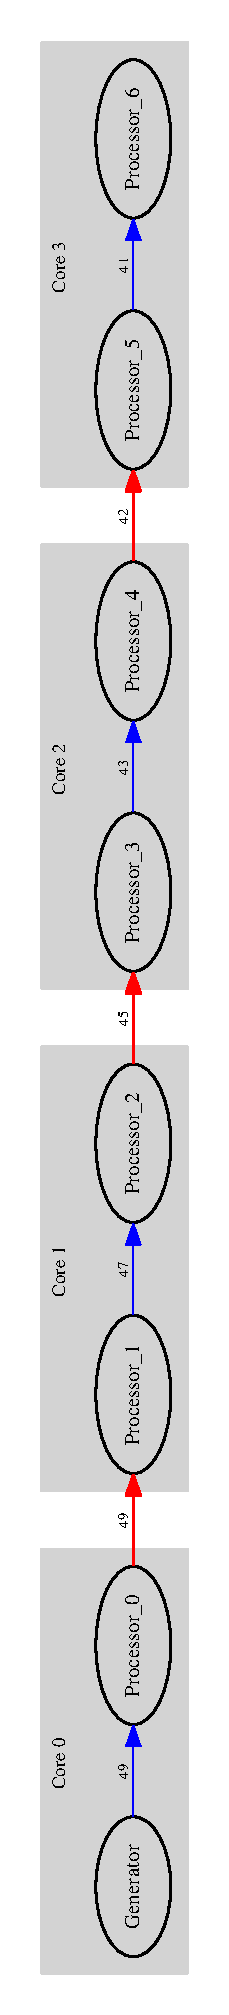
\includegraphics[height=\textwidth, angle=-90 ]{fig/queue_allocation.eps}
    \caption{Queue model simulation trace across 4 kernels.}
    \label{fig:Queue_allocation}
\end{figure*}
\begin{figure}
    \center
    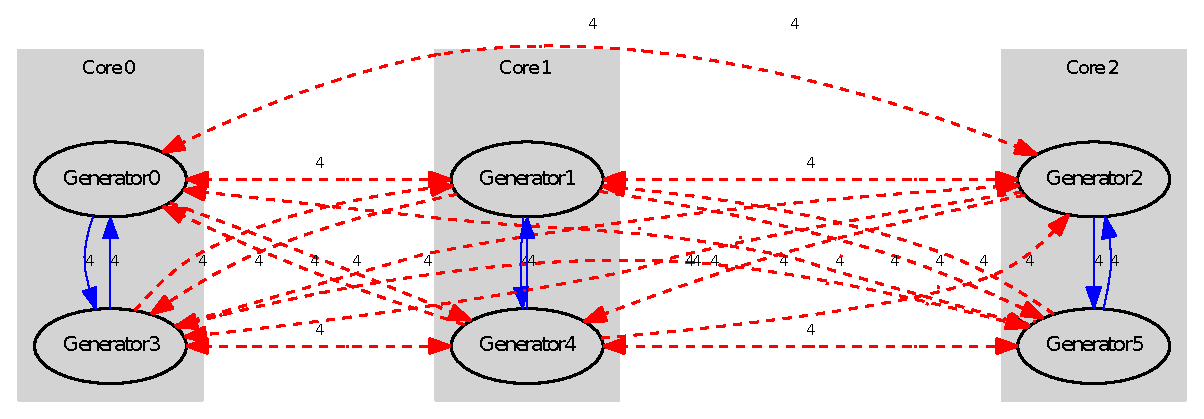
\includegraphics[width=\plotfraction\columnwidth]{fig/interconnect_parallel_allocation.eps}
    \caption{Interconnect simulation trace for 6 models on 3 kernels.}
    \label{fig:interconnect_allocation_parallel}
\end{figure}
\begin{figure}
    \center
    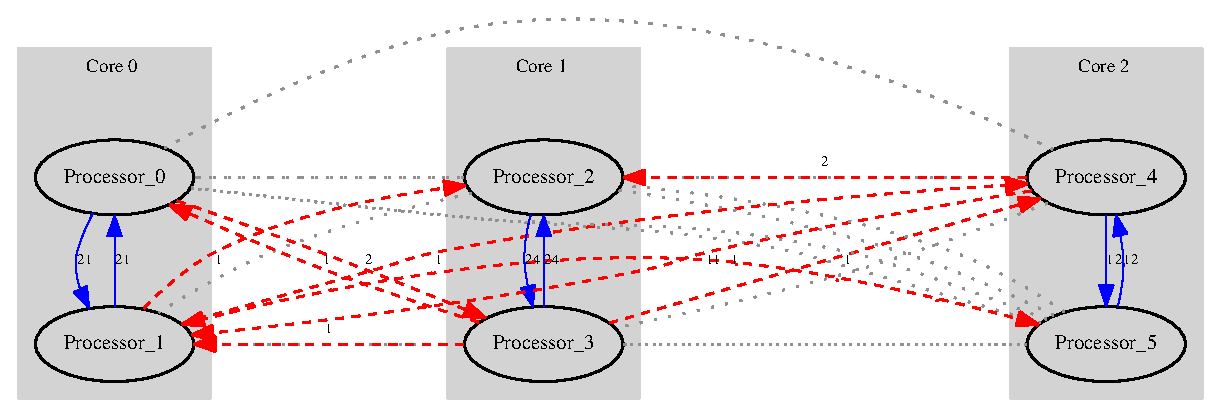
\includegraphics[width=\plotfraction\columnwidth]{fig/phold_parallel_allocation.eps}
    \caption{Phold simulation trace for parallel simulation using three kernels.}
    \label{fig:phold_allocation}
\end{figure}
